\section{Software}
%\subsection{Description}
The software of this project contains 3 parts:
\begin{itemize}
\item{The operating system configuration and modification to be fully compatible with the hardware used.}
\item{The website that is used by the young users to send pictures and messages to the old users.}
\item{The Vesta tab software that is used on the tablet to display the differents messages and pictures received by the old users.}
\end{itemize}

The figure \ref{fig:web connections} shows the web interactions between the website and the Vesta software on the tablet.

\begin{figure}[!htb]
    \centering
    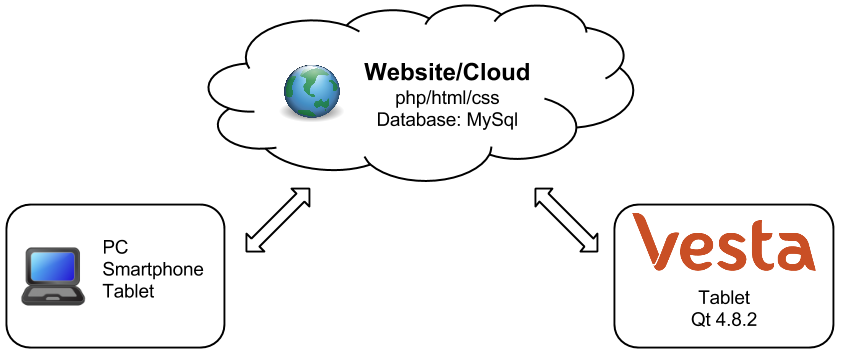
\includegraphics[width=0.9\textwidth,keepaspectratio]{chap/softFig/web_connections.png}
    \caption{Web connections}
    \label{fig:web connections}
\end{figure}

The figure \ref{fig:user flow} shows the interactions between the website and the Vesta software on the tablet. All the files are stored on the website on the mySql database. When the pictures are sent, the vesta tablet receives a message and can open/display it. The vesta software on the tablet works on a linux OS that manages the hardware.

\begin{figure}[!htb]
    \centering
    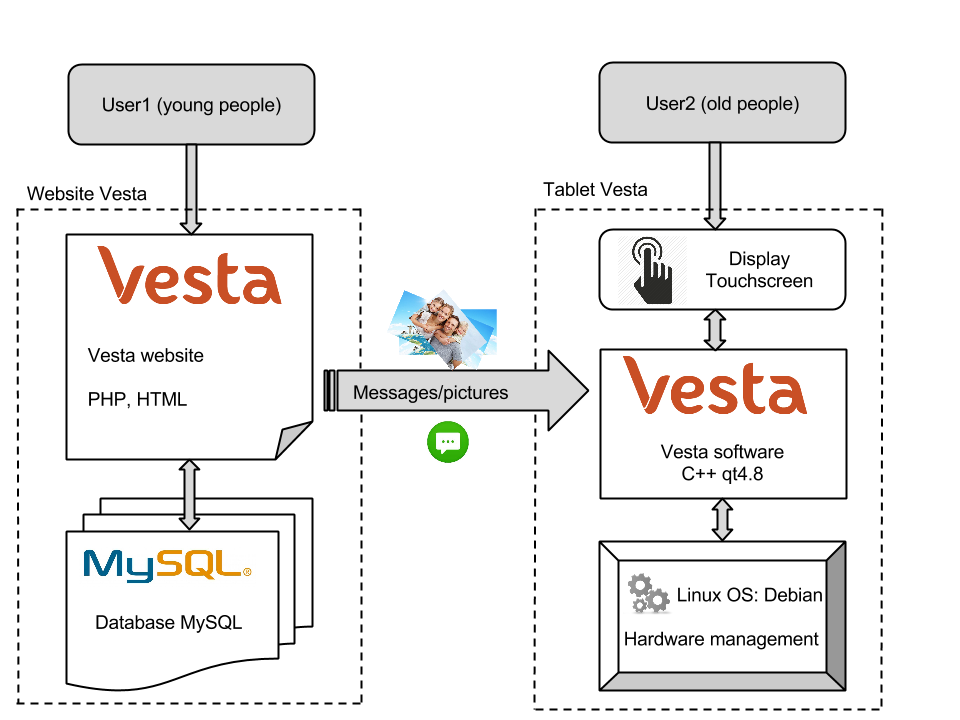
\includegraphics[width=0.9\textwidth,keepaspectratio]{chap/softFig/block_diagram_vesta2.png}
    \caption{Basic user flow.}
    \label{fig:user flow}
\end{figure}

\subsection{Operating system}
The OS used for this project is a debian. Debian is a linux distribution and was given by the conceptors of the beaglebone black. The OS manage the communications with the different hardware. The accelerometer is controled by I2C (to read datas and write configurations). The screen uses different interfaces, I2C for the touch panel and 24bit parallel for the display. The WIFI chip is connected with SDIO and it replace the emmc memory.

Every protocol and every pins input or output have to be declared in a file called device tree source. In the 3.14 kernel, this file is compiled and become a device tree blob. The compiled version of the file is executed at the OS startup. It initiates the load of the drivers and configures the pins as input, output, pwm or interrupt. Some pins can be configured as i2c, spi, SDIO or some other protocols.

\subsubsection{Drivers}
A lot of work on this linux distribution was made to be fully compatible with the chosen hardware.
The touch screen driver edt-ft5x06 had problems with the original 3.8 kernel of the distribution we used. The driver was not loading correctly from the device tree overlay. An upgrade to the 3.14 kernel resolved the problem.
Then the scale of the touchscreen was not correct. 
When a touch event was done on the right-down corner, the mouse pointer moved to the center of the screen. Some configuration scripts had to be modified for the X11 graphical display server.

The edt-ft5x06 uses an interrupt line and I2C to get the touch events and the positions of the clicks.

Another driver is used for the WIFI connection with the wl1835mod. This driver uses the protocol SDIO. It also has to be declared and initialized at the OS startup in the device tree blob. As the beaglebone's processor has only one SDIO protocol possible and it is used be the emmc memory, the emmc is replaced by with WIFI chip and the emmc is unusable.

\subsubsection{Display}
The touch screen works with a 24 bits parallel interface so the X11 configuration file had to be modified to work correctly. The LCD output was initialy configured in 16 bits parallel interface.
The hardware management in linux is called a device tree blob. It’s a script that is compiled and is loaded at the OS startup. In this file, the driver for the touch panel was declared and the interrupt pins was defined. The resolution and frequency of the display is also configured in this script. The wifi chip also needs to load drivers at startup and tell the OS to connect to internet via this chip and with the SDIO protocol.
The file is located in /boot/dtbs/3.14xx/ and is called vesta.dtb (compiled) and the source is called vesta.dts. The file uEnv.txt located in /boot/ also need to define which device tree blob(dtb) the OS has to load at startup.
\begin{figure}[!htb]
    \centering
    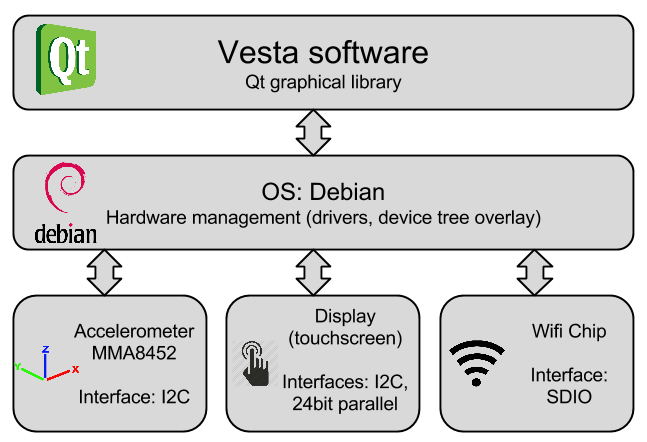
\includegraphics[width=0.9\textwidth,keepaspectratio]{chap/softFig/first_diagram2}
    \caption{Firmware dependencies.}
    \label{fig:firmware dependencies}
\end{figure}

\subsection{Website}
The website is used by the young users to send messages and pictures to the old user’s tablet.
The website contains a MySQL database, a php/html page that let the young user send a message and a php script used to parse the database to XML to be readable by the tablet.

\begin{figure}[!htb]
    \centering
    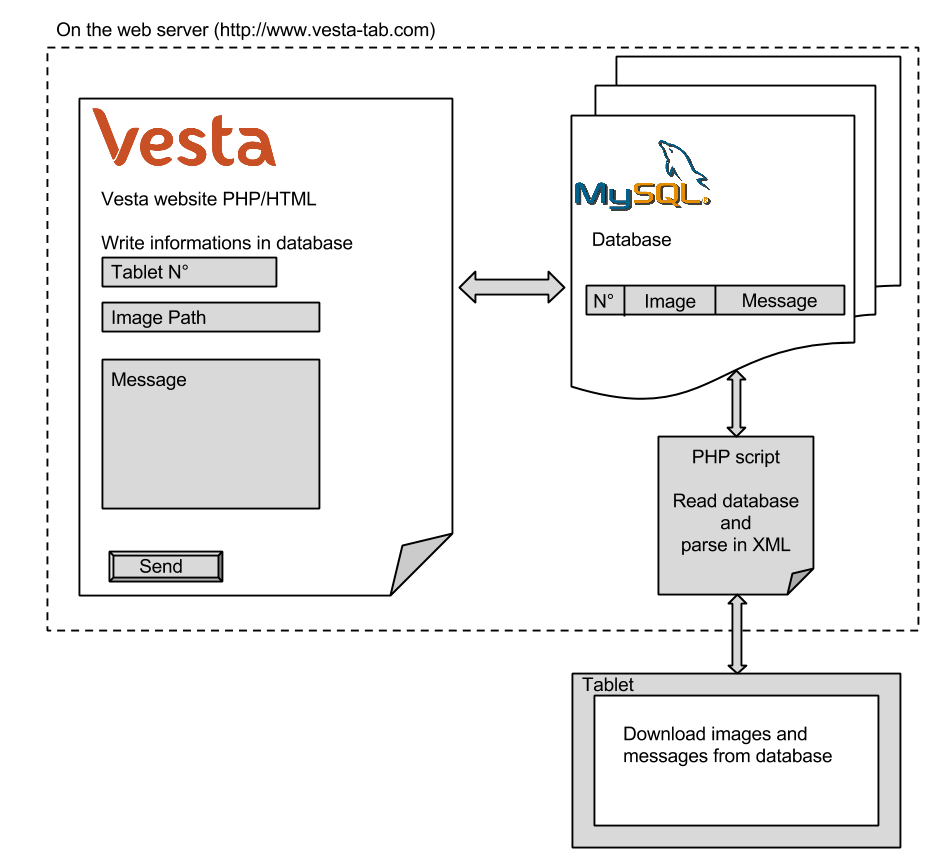
\includegraphics[width=0.9\textwidth,keepaspectratio]{chap/softFig/vesta_website2}
    \caption{Vesta website architecture.}
    \label{fig:web archi}
\end{figure}

\subsubsection{Webpage}
The webpage let the young user send a message to a wanted tablet. Every tablet has an id like a phone number known by the tablet owner. It is possible to select a picture on the user's computer and write a text message. When the "send" button is clicked, the picture and text message is saved in the MySQL database.

The php script called when the send button is clicked downloads the picture contained in the file input, verify if the file downloaded is a picture and if the size is not too big. If everything went well the picture and the other datas are saved in the MySQL database else some error messages are displayed. The date is automatically written at the current time.

\subsubsection{Database and XML parsing}
The MySQL database is where all the messages and pictures are stored. The webpage connects and save the datas into the database when the user send a message.

An example of entries on the vesta table on the MySQL database are shown in the table\ref{tab:database}.

\begin{table}
\begin{tabular}{|c|c|c|c|c|c|}
  \hline
  id & type & name & text & img & date \\
  \hline
  7 & image/jpeg & family.jpg & Hello! A message for you & BLOB - 300KB & 14.05.2015 13:23:43 \\
  8 & image/jpeg & cat.jpg & Look at my cat :) & BLOB - 350KB & 27.05.2015 18:10:05 \\
  \hline
\end{tabular}
\caption {Example of entries in the vesta table on the MySQL database}\label{tab:database}
\end{table}

When the tablet update the datas, it connects to a script contained on the server. This script connects to the database and parse the informations needed by the tablet in XML.The tablet then unparse the datas, downloads the pictures, and display them.

XML is a markup language that facilitates the transfer of datas and the readability of them. It is mainly used in the RSS flux.


The XML code look like this:

<?xml version="1.0"?>
<vesta>
  <item>
    <title>family.jpg</title>
    <image>http://www.vesta-tab.com/jo/getImage.php?id=7</image>
    <message>Hello! A message for you</message>
  </item>
  <item>
    <title>cat.jpg</title>
    <image>http://www.vesta-tab.com/jo/getImage.php?id=8</image>
    <message>Look at my cat</message>
  </item>
</vesta>

\subsection{Vesta software}
The Vesta software is used by the old users to receive and display the messages and pictures sent by the young users. It is located on the tablet and working with debian. The software is made in C++ with Qt4.8/Qt quick 1.0.

\subsubsection{Qt library}
Qt is a free library used mainly to design softwares with graphical user interfaces (GUI). It is cross platform so with the same code it is possible to compile for linux,windows and mac.
The library contains also a lot of utils to facilitate the development of emmbedded interfaces and manages the touchscreen events like the swipes, clicks and more. A lot of documentation is available and a lot of users develop with it.

There are differents GUI library like Gtk+, CEGUI etc... The choice of Qt was done especially because it is cross platform but also because it's compatible with emmbedded systems. Qt can be used also with android and IOS and is really made for apps with touchscreen. Qt quick is very powerful for emmbedded applications. The last version of Qt was downloaded over 1 million times and is ranked number 1 of all cross-platform tools.

\subsubsection{Overall operations}
At the startup, the vesta tab init and check the wifi connection. The touchscreen creates an event when someone touch it and changes the image displayed. It lets the user naviguate between the different messages. Every minute the soft check if a new message is received.

The software is quite simple and not a lot of functionnalities are implemented. The goal was to have a really easy to use software for old people.

The figure \ref{fig:soft archi} shows how the software works.

\begin{figure}[!htb]
    \centering
    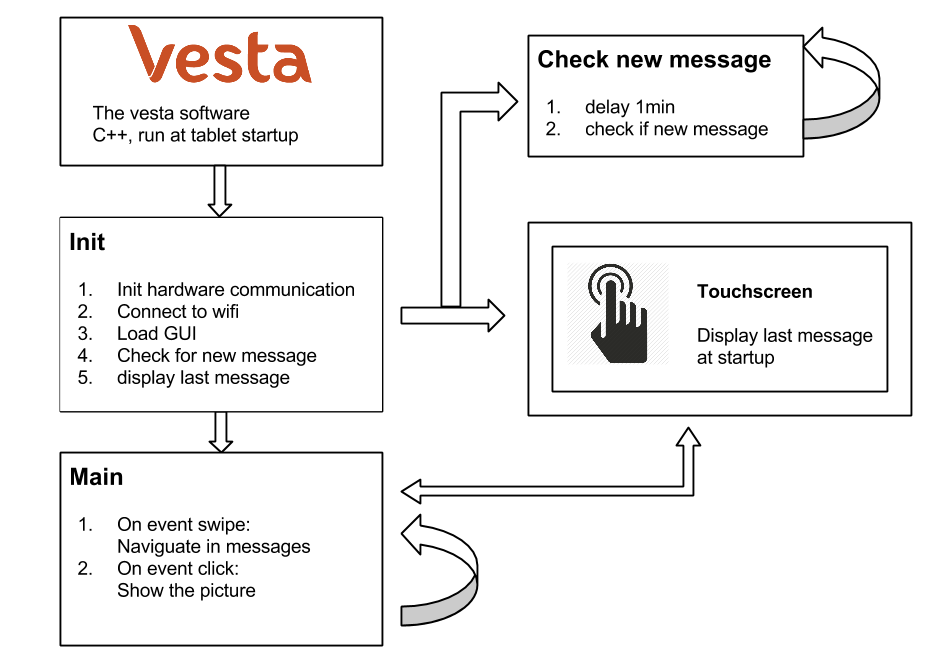
\includegraphics[width=0.9\textwidth,keepaspectratio]{chap/softFig/vesta_software_diagram2}
    \caption{Vesta software architecture.}
    \label{fig:soft archi}
\end{figure}

\subsubsection{Graphical interface}
The graphical interface is composed of an horizontal listview and some buttons. The listview allows swipes event to naviguate between the different pictures and messages.

A task bar is always visible on the top of the GUI. The list view displays the actual picture, the date when the messages was sent and the text message.

The buttons let the user configure the wifi or display the new messages.

\begin{itemize}
\item{The button A refresh the messages and display the last one.}
\item{The button B goes to the WIFI configuration and indicates the RSSI of the WIFI.}
\item{The indicator C show the battery level}
\end{itemize}

The figure \ref{fig:gui diagram} shows how the GUI is constructed.

\begin{figure}[!htb]
    \centering
    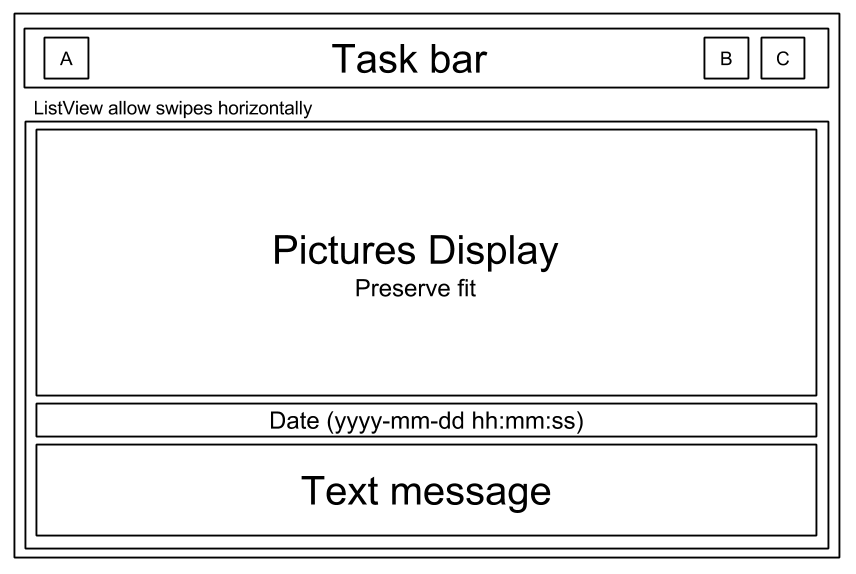
\includegraphics[width=0.9\textwidth,keepaspectratio]{chap/softFig/GUI_diagram}
    \caption{Graphical interface diagram, A:Refresh button, B:WIFI RSSI indicator, C:Battery state indicator}
    \label{fig:gui diagram}
\end{figure}

The figure \ref{fig:graphical interface} shows the actual GUI.

\begin{figure}[!htb]
    \centering
    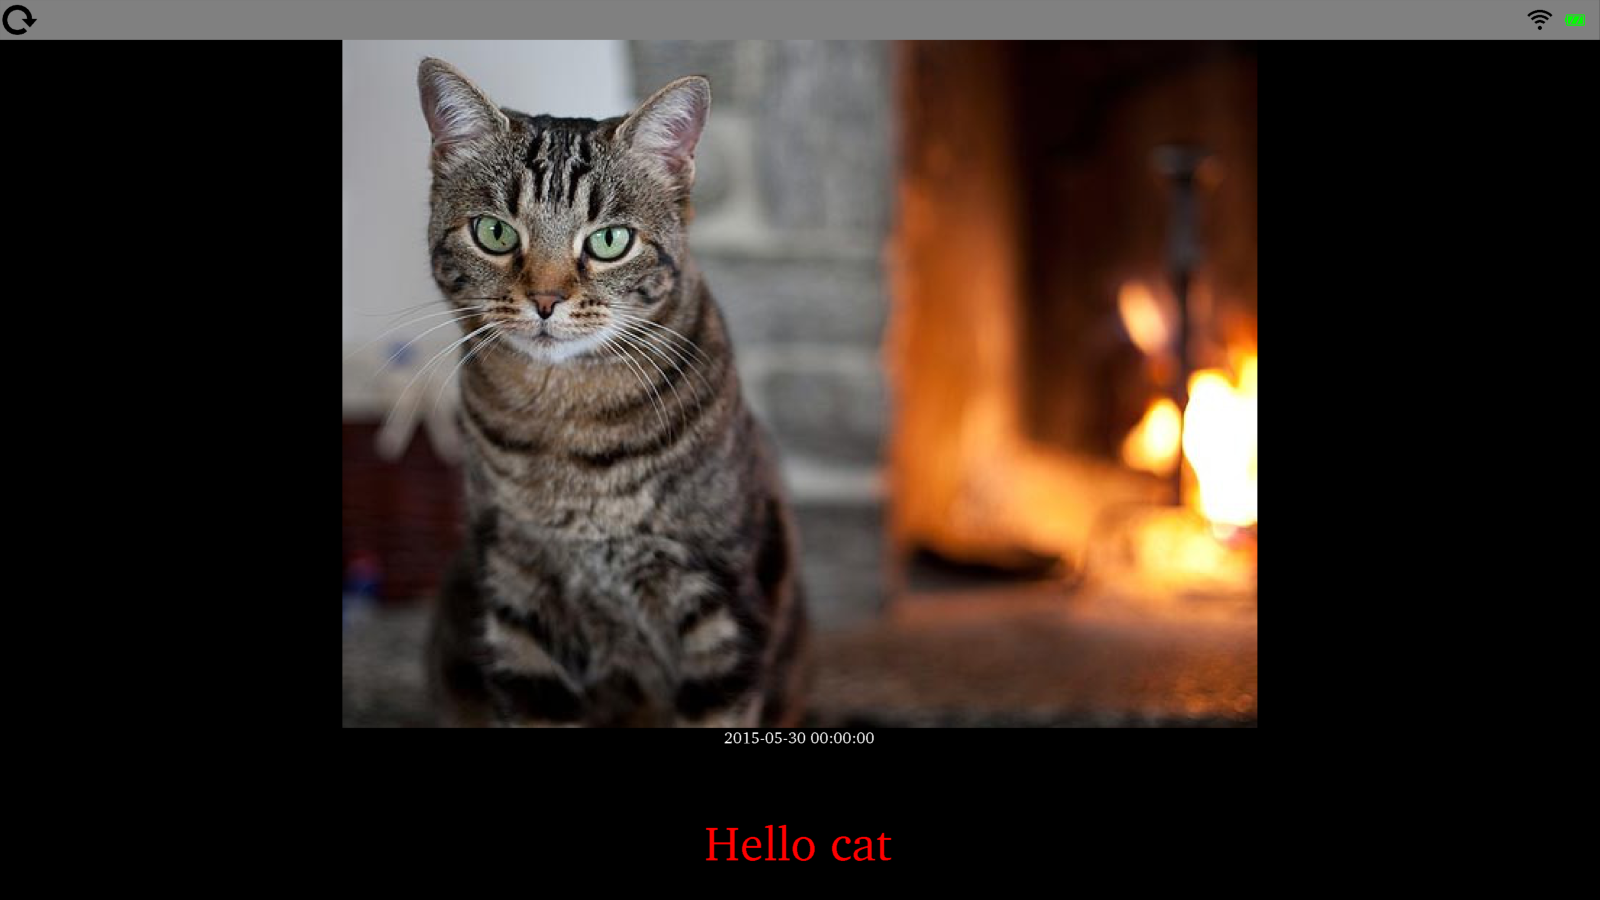
\includegraphics[width=0.9\textwidth,keepaspectratio]{chap/softFig/vesta_printscreen}
    \caption{Vesta software graphical interface}
    \label{fig:graphical interface}
\end{figure}


